\begin{frame}
	\frametitle{PHEW}
	
%	\begin{columns}
%		\column{.6\textwidth}
			\begin{itemize}
				\item \phew\ groups cells together by separating the mass density field along minima, thus dividing the density field into patches.
				
%				\item The density field is obtained with the deposition of the particle’s mass on the mesh through ``Cloud in Cell'' interpolation.
				
				\item The algorithm can	be divided in four main steps:
				
				\begin{itemize}
					\item segmentation
					\item connectivity establishment
					\item noise removal and
					\item substructure merging
				\end{itemize}
			\end{itemize}
%		\column{.4\textwidth}
%			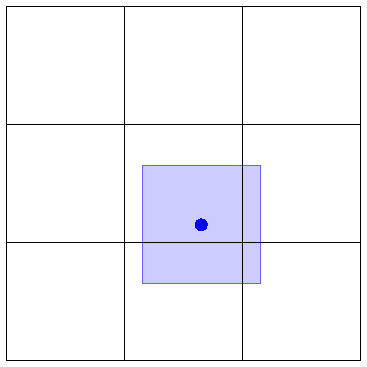
\includegraphics[width = \textwidth, keepaspectratio]{images/tikz/CIC.pdf}
%	\end{columns}
	  
\end{frame}


%\begin{frame}
%	\frametitle{Segmentation}
%	\begin{itemize}
%		\item First, all overdense cells (``test cells'') are identified. If a cell does not have a denser neighbour cell, it is marked as a local density peak and assigned a peak label.
%		
%		\item Then each test cell copies the peak label of its densest neighbour. This way, each cell is assigned
%		to the peak “closest” to it by following the path of rising density.
%		
%		\item All test cells assigned to a particular peak form a peak patch. The separating surface between peak
%		patches will be cell borders which contain local density minima.
%	\end{itemize}
%\end{frame}
%
%\begin{frame}
%	\frametitle{Connectivity Establishment}
%	
%	\begin{itemize}
%		\item For each peak patch, all neighbouring peak patches are identified.
%		The maximal surface density between two particular peak patches is considered as the “saddle” between these two.
%		
%		\item For each peak, out of all the saddles of all the neighbouring peak patches, the one with the highest density is called the “key saddle” and the neighbour it connects to is referred to as the “key neighbour”.
%	\end{itemize}
%	
%\end{frame}
%
%\begin{frame}
%	\frametitle{Noise Removal}
%	\begin{itemize}
%		\item Each peak patch is assigned a value representing the contrast to the background
%		called “relevance”. A peak patch’s relevance is defined as the ratio of the peak’s density to the density of its key saddle. 
%		
%		\item A peak patch is considered noise if the its relevance is lower than a user-defined relevance
%		threshold. 
%		
%		\item An irrelevant peak patch is then merged into its key neighbour or discarded if it has no neighbours.
%		
%		\item Once the noise removal step is completed, the remaining structure consists only of peak patches
%		which satisfy the relevance condition and is referred to as “level 0 clumps”. These clumps represent the structure on the lowest scale.
%	\end{itemize}
%\end{frame}
%
%\begin{frame}
%	\frametitle{Substructure Merging}
%	\begin{itemize}
%		\item The identified level 0 clumps can be merged further into composite clumps.
%		
%		\item All peak patches whose key saddle density is
%		higher than the user-defined threshold are merged into their key neighbour. 
%		
%		\item The saddle threshold defines which clumps should be considered as separate structures and which should be merged and considered as composite structures.
%		
%		\item Because the peak patches grow when merged, new connections between peak patches that weren't neighbours before are created.
%		The merging step can be repeated until no more merging can occur. Each merging loop then represents a different level of substructure: In each loop, greater structures are being merged into each other than there were in the loop before. 
%	\end{itemize}
%\end{frame}


\begin{frame}
	\centering
	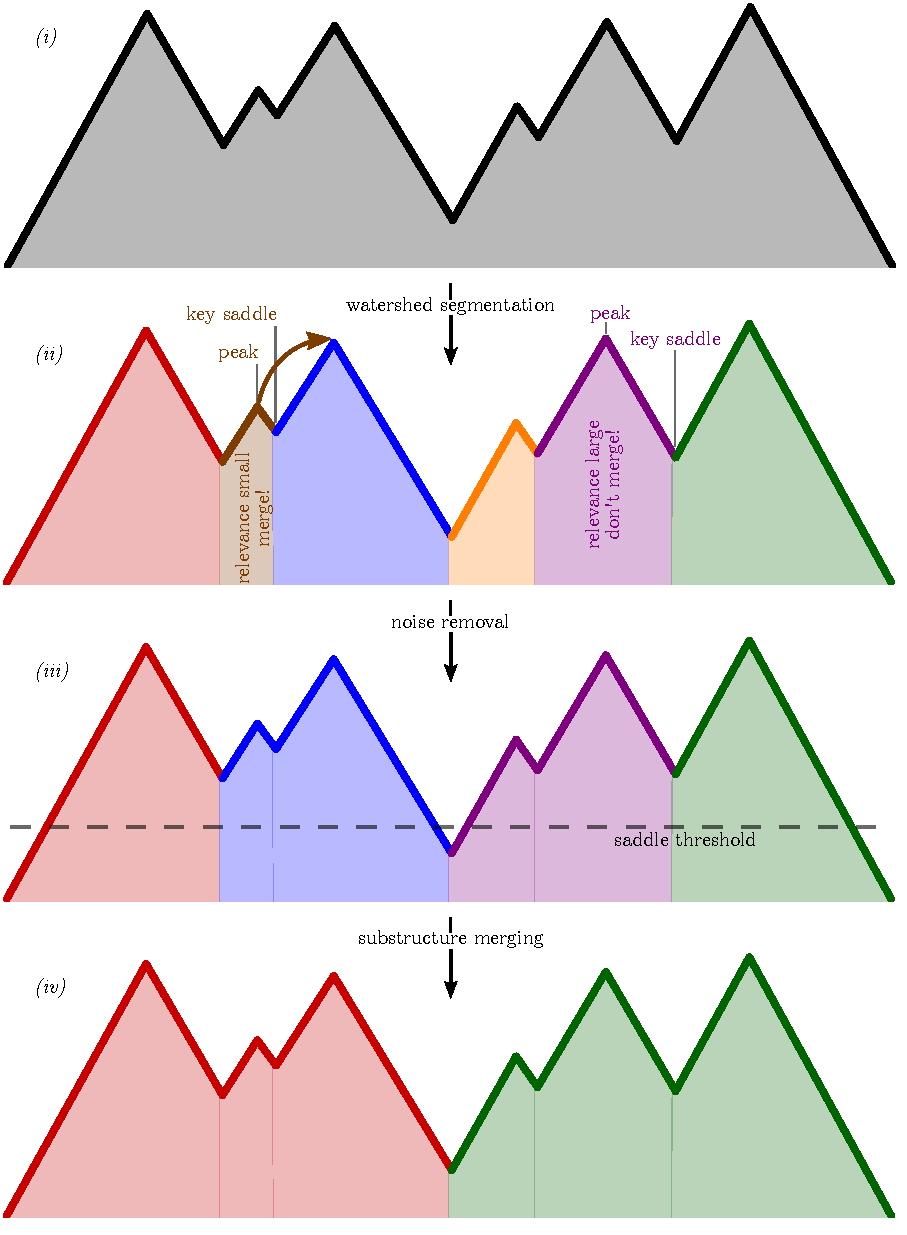
\includegraphics[height=.95\textheight]{../report/images/phew/soap.pdf}
	
	{\tiny Image adapted from \cite{PHEW}.}
\end{frame}